%\chapter{IG Knowledge Models}
\section{\uppercase{IG Knowledge Models}}
This section details our ontology (IGO). Due to the large number of concept/classes we first reorganized the governance classification scheme into 6 top level categories and 26 sub-categories. For each top-level category we created an ontology. 
The top-level categories are: Organization (ORG), Information (INF), System (SYS), Component (CPT), Lifecycle (LCS) and Platform (PLT). We then harmonized the vocabulary terms and aligned them according to their implementation relevance and the functional area they belong to. Each sub-category consists of a number of requirements, capabilities, recommendations and domain constraints. Together they form the overall IGO concept model. A bird’s perspective of the IGO graph was presented in Figure 3 a few more details are discussed next. 
%\paragraph{}
The foundational ontology is Organization. It is composed of the child level categories: Agent, Goal, Objective, Quality, Compliance and Responsibility. They form the high-level concepts, a semantic graph that represent an Organization and its associated concept classes in our context.  Each class has a description, relations (object properties), attributes (data properties), comments and annotations. We synthesized this information from domain knowledge, best practices, and guidelines. (not shown in this paper). The use of formal description ensures that concept descriptions utilize unambiguous semantics and well-formed rule sets readable by both machines and humans. The following 6 sub-sections provide a high-level overview of the 6 ontologies created.
%%
%\vfill
\subsection{Organizational Model(ORG)}
Model Description: Figure 5 shows the top-level concepts of an organization as a semantic graph. The defined concepts are: Organization, Organizational Unit, Enterprise, Department on the right side. Governance, Governing Body and Steering Committee on the left side. One level below you see instances of Organizational Unit: Business, Legal, Records Management, Architecture and IT. These are the typical Departments in an Enterprises. 
%
\begin{figure}[h]
  \centering
    \includegraphics[width=7.5cm]
%    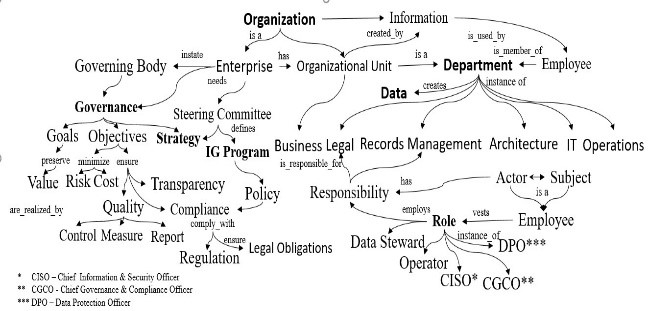
\includegraphics[clip,trim=1cm 7cm 0 0,width=7.5cm]
    {images/Fig5-IG.Org.Model.png}
    \caption{Organization design model (ORG)}
  \label{fig:orgmod}
\end{figure}
% //Figure 5: Organization semantic model (ORG).
The idea conveyed is that departments produce Data and Metadata through their services. Steering Committees define long term goals and short-term objectives. The latter being: data quality, compliance with regulations and legal obligations. The lower right corner of Figure 5 lists Employees who vest Roles that are associated with Responsibilities and their employed duties. Relevant governance related roles are: CGCO , CISO , and DPO .
%\vfill
\subsection{Information Model(INF)}
Model Description: The Information ontology (INF) is constructed around the key concept of Data. The graph lists the concepts like: Content, Metadata and Asset as derived classes. They represent digital objects of any type and format. In this model, an Asset represents a data container that links (aggregates) together digital content, its metadata and associated contextual information. At concept level Information is shown as being derived from Metadata which is itself derived from data. Figure 6 shows the governance management model, starting with the key concept of Record and its relation to Data. A Record represents a set of governance metadata consisting of classification information used to define process control information related to security, privacy, retention and disposition. Such processes are controlled by Policy instances containing Rules specific to the data category and lifecycle phase in which data is being processed. 
From a governance standpoint, the concept of a Policy is the control mechanism assigned to data through a Record. The record metadata reflects its classification, according to applicable taxonomies.
%
\begin{figure}[h]
  \centering
    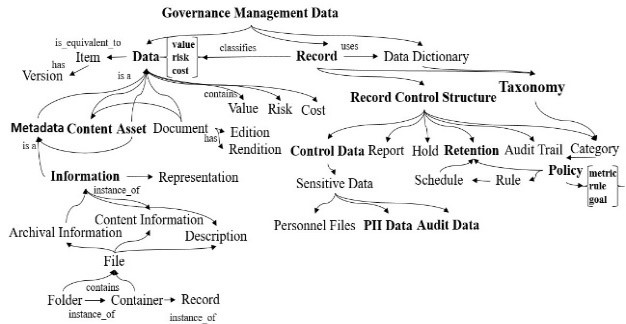
\includegraphics[width=7.5cm]{images/Fig6-IG.Inf.Model.png}
    \caption{Information design model (INF).}
  \label{fig:infmod}
\end{figure}
By definition, a Policy class aggregates goals, rules and metrics and is used by an information governance Lifecycle. Goals, Rules and Metrics depended on whether it refers to Content, Metadata, Asset, Records or collateral Information. Assets have value, cost and risk. Characteristics that are controlled by governance policies. Policies employ the rules used to steer wanted information governance course. Typically, access to persisted data is secured by a security policy in a way that data objects are assigned access control permissions and roles are given a set of privileges i.e. rights. To a subject requesting to retrieve a specific data object, access is granted if the subject vests a Role, where the roles privileges do match the permission assigned to the data object. 
Value, cost and risk of data depend on time; therefore, the applied policies must change over time and thus require an ongoing process that adjusts policy rules accordingly. Typical data storage rules are R1) Data with no value V (t) =0 and must be deleted to reduce cost; R2) Data with high value must be kept forever, but to reduce cost it has to be moved onto less expensive storage. R3) PII Data must be stored and handled according to regulations by jurisdiction. 
%
%\vfill
\subsection{System Model (SYS)}
Model Description: The Systems semantic model entails the core concepts of the implementation domain (see Figure 3). The vocabulary terms used in this model, reflect key concepts related to the architecture and design of an IG solution that are based on requirements related to the IG program and its implementations. Top-level classes are Architecture, Design, Model and model instances, including: Data- and Information Model down to the deployment and execution model.
 The architecture and design terms listed in Figure 7 represent system characteristics typical of Enterprise Information System (EIS). The semantic schema outlined, shows the relationships between architecture and systems components. It explains what they do and how to use them. The lower part of Figure 7 models the internal structure of an EIS system. Consisting of a number of service components like: Content-, Information Retrieval- and Analytics components. A Repository in turn utilizes a Catalog and a Full Text Index as its source of information. Last in this hierarchy is the Execution Environment and the Platform, concepts native to the IaaS domain that describe how infrastructure resources of the type Compute, Network and Storage are provisioned or de-provisioned.
%
\begin{figure}[h]
  \centering
    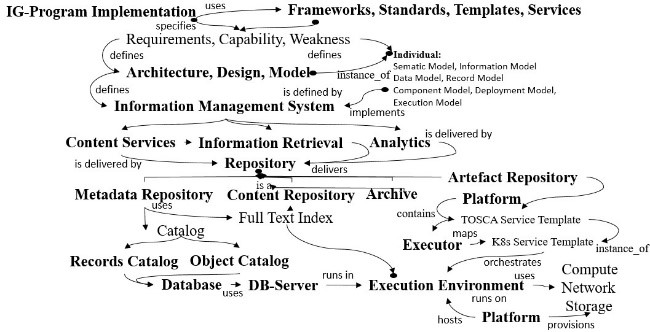
\includegraphics[width=7.5cm]{images/Fig7-IG.sys.Model.png}
    \caption{System design model (SYS).}
  \label{fig:sysmod}
\end{figure}
%\vfill
\subsection{Component Model(CPT)}
Model Description: The Component ontology shown in Figure 8 is about concepts corresponding to the major functional areas covered by an IG framework These areas cover: Administration, Maintenance, Management, Security, Privacy, Function, and Records. Addressing functions like: Collect, Store, Access, Index, and Classify components that represent software with those capabilities. Through the IGONTO framework (see Figure 11), these concept/classes are mapped to pre-existing software services. We found many of these services provided online. 
Their consumption is modelled as service junction-points. A model that allows to form cross-platform data processing pipelines.
%Component design model (CPT).
%
\begin{figure}[h]
  \centering
    \includegraphics[width=7.5cm]{images/Fig8-IG.CPT.Model.png}
    \caption{Component design model (CPT).}
  \label{fig:cptmod}
\end{figure}
%
%\vfill
\subsection{Lifecycle Model(LCS)}
 Model Description: The governance Lifecycle model aggregates concepts related to services and processes bound to workflows that steer the data processing chain. They enforce corporate governance policies using appropriate methods along the process pipeline (see Figure 1) to collect records metadata.
%
%Lifecycle Model (LCS).
%
\begin{figure}[h]
  \centering
    \includegraphics[width=7.5cm]{images/Fig9-IG.LCS.Model.png}
    \caption{Lifecycle design model (LCS).}
  \label{fig:lcsmod}
\end{figure}
Governance lifecycles protocol aspects on how data processed. The governance logic monitors the process flow and how data handled in their business production environment. Along the data processing pipeline complementary tracking information is produce to ensure and safeguard the chain of custody.
%
%\vfill
\subsection{Platform Model(PLT)}
Model Description: The Platform ontology (PLT) models the platform level. It describes the execution environment, in which a system, its component and required infrastructure resources are deployed and orchestrated. Figure 9 
%Platform design model (CPT).
%
\begin{figure}[h]
  \centering
    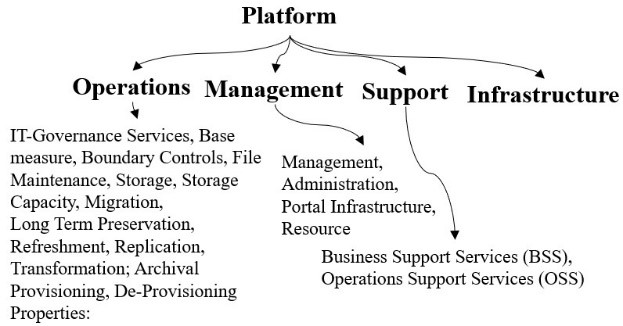
\includegraphics[width=7.5cm]{images/Fig10-IG.Plt.Model.png }
    \caption{Platform design model (PLT).}
  \label{fig:pltmod}
\end{figure}
% \vfill
For this ontology we collected descriptions of available TOSCA service templates, their capabilities and relationships. Such a service template describes at concept level the required infrastructure resources, the runtime environment, the build plans (implementation artifacts) and the orchestration logic. Usage notes complements the service templates with the instruction of how to map a TOSCA services template to a platform specific service instance. 
For this research we used several tools and technics that yielded the GONTO framework as a byproduct, shown in Figure 11. We used Microsoft Excel to design the taxonomies and prepared the data to create concept models. The formalized knowledge helped defining our ontology. Protégé (Musen, 2015)is used as the primary ontology authoring tool. Apache Jena for loading of the data into the AllegroGraph (AGraph) triple store. Apache Fuseki is the protocol used to execute SPARQL queries for both reporting as well as updating the triple stores. Gruff as the tool for viewing, querying and manipulating elements of the semantic data (IGG).